%
% speziell.tex -- Spezielle Relativitätstheorie
%
% (c) 2017 Prof Dr Andreas Müller, Hochschule Rapperswil
%

\chapter{Spezielle Relativitätstheorie%
\label{skript:chapter:spezielle}}
\lhead{Spezielle Relativitätstheorie}
\rhead{}
Im 19.~Jahrhundert hat James Clark Maxwell die Theorien
über Elektriztität und Magnetismus zu einer einheitlichen Theorie
der Elektrodynamik zusammengefasst.
\index{Maxwell, James Clark}
\index{Elektrodynamik}
Diese Theorie ist die Grundlage aller Phänomene, mit denen sich
ein Elektroingenieur täglich herumschlägt.
Sie kann daher als mit herausragender Präzision bestätigt gelten.
Zum Beispiel beschreibt sie die Ausbreitung von elektromagnetischen
Wellen wie Licht oder Radiowellen, erklärt aber nicht das Medium, in
dem diese Wellen sich ausbreiten.
Der gescheiterte Versuch, ein solches Medium nachzuweisen, hat zu einer
der tiefgreifendsten Umwälzungen unseres Weltbildes geführt.

\section{Galilei-Transformation}
\rhead{Galilei-Transformation}
Die Mechanik kann zwischen Ruhe und gleichförmiger Bewegung nicht 
unterschieden.
Mit mechanischen Experimenten kann man ein Labor, welches weit von
allen Sternen entfernt im Universum schwebt nicht von einem ähnlichen
Labor unterschieden, welches sich mit einer Geschwindigkeit von 1000m/s
relativ dazu bewegt.
Um dies genauer verstehen zu können, verwenden wir in dem ruhenden Labor
Koordinaten $(t,x)$ und dem relativ dazu mit Geschwindigkeit $v$ bewegten
Labor die Koordinaten
$(t',x')$\footnote{Wir arbeiten hier der Einfachheit halber nur mit einer
einzigen Raumkoordinate.
Der physikalische Raum hat natürlich deren drei, man kann dies erreichen,
indem man sich $x$ und $x'$ als dreidimensionale Vektoren vorstellt.}.
Die Umrechnung zwischen den Koordinaten betrifft nur die Ortskoordinaten,
wir erwarten daher, dass die Umrechnung zwischen den Koordinatensystemen
mit den Formeln
\begin{equation}
\begin{aligned}
t'&=t\\
x'&=x+vt
\end{aligned}
\label{skript:kruemmung:galileitransformation}
\end{equation}
\index{Galiei-Transformation}
Man nennt \eqref{skript:kruemmung:galileitransformation} die
Galilei-Transformation.

Wir betrachten jetzt die Beschreibung eines bewegten Körpers in diesen
Koordinaten.
Die Bahn des Körpers wird durch eine Funktion $x(t)$ in $(t,x)$-Koordinaten
beschrieben.
In $(t',x')$-Koordinaten wird nach der Galilei-Transformation daraus
$t'=t$ und $x'(t')=x(t)+vt$.
Die Bewegung wird bestimmt durch die Kräfte, nach dem zweiten Newtonschen
Gesetz also durch die Beschleunigung:
\begin{align}
\dot x'(t')
&=
\frac{dx'(t')}{dt'}
=
\frac{d}{dt}(x(t)+vt)
=
\dot x(t) + v
&&\Rightarrow&
\ddot x'(t')
&=
\frac{d^2x'(t')}{dt'^2}
=
\frac{d}{dt} (\dot x(t) + v)
=
\ddot x(t).
\end{align}
Die Beschleunigung und damit die Kräfte unterscheiden sich also in den
beiden Koordinatensystemen nicht.
Das zweite Newtonsche Gesetz gilt daher in ruhenden wie in bewegten
Laboratorien gleichermassen, es kann nicht dazu verwendet werden, zwischen
Ruhe und Bewegung zu unterscheiden.

Dies ändert sich plötzlich, wenn elektrische und magnetische Phänomene
ins Spiel kommen.
Eine ruhende Ladung erzeugt ein elektrisches Feld, welches eine Magnetnadel
nicht beeinflussen kann.
Sobald sich die Ladung bewegt, entsteht zusätzlich ein magnetisches Feld,
welches von der Magnetnadel detektiert werden kann.
Man kann daher keine voll\-ständige Beschreibung dieser Phänomene erwarten,
solange man nicht beide in einer einzigen Theorie, der sogenannten
Elektrodynamik zusammenfasst.

Diese Theorie sagt Wellen voraus, die wir als Licht oder auch als Radiowellen
täglich nutzen.
Im 19.~Jahrhundert lag die Vermutung nahe, dass es ein Medium gibt,
den sogenannten Äther, welches
diese Wellen transportiert, und dessen Geschwindigkeit gemessen werden
kann, so wie man bei einer Schifffahrt die Geschwindigkeit des Wassers
messen kann, welches auch Wellen transportiert.
Wenn diese mechanische Betrachtungsweise der Lichtwellenausbreitung
zutrifft, dann müsste die gemessene Lichtgeschwindigkeit von der
Geschwindigkeit abhängen, mit der sich ein Labor relativ zum Medium
bewegt.
Bewegt sich das Medium mit Geschwindigkeit $v$, erwartet man die
Lichtgeschwindigkeit $c+v$, wenn sich das Licht in die gleiche Richtung
bewegt, und $c-v$, wenn es sich in entgegengesetzer Richtung bewegt.

Ein grundlegendes Problem für die Elektrodynamik ist, dass die
Formeln der Theorie sich ändern, wenn man auf die Koordinaten eine
Galilei-Transformation anwendet.
Eine Messung der Geschwindigkeit des Äthers würde also gleichzeitig
zeigen, dass die Formeln der Elektrodynamik nicht voll\-ständig sind,
dass es eine Version davon geben muss, die mit der Galilei-Transformation
verträglich ist.

Findet man den Äther dagegen nicht, und stellen sich keine anderen Gründe
ein, an der Korrektheit der Elektrodynamik zu zweifeln, dann ist damit
die universelle Anwendbarkeit der Galilei-Transformation 
\eqref{skript:kruemmung:galileitransformation} in Frage gestellt.
Diese intuitiv einleuchtende Transformation kann dann nur noch eine
Approximation sein, deren Fehler bisher nur deshalb nicht aufgefallen
sind, weil sie erst bei sehr grossen Geschwindigkeiten sichbar werden.

\begin{figure}
\centering
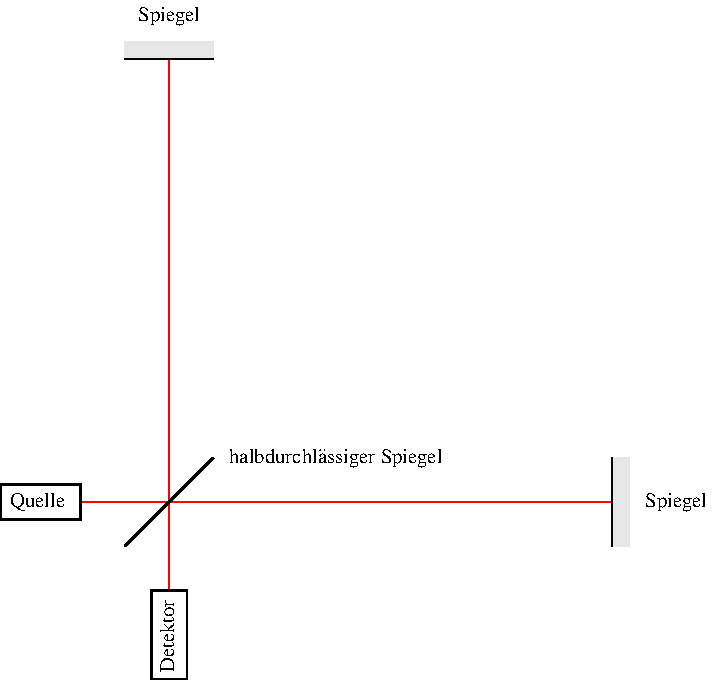
\includegraphics{chapters/tikz/interferometer.pdf}
\caption{Schematische Darstellung des Interferometers von Michelson und Morley.
Die beiden Arme des Interferometers sind gleich lang, so dass das Licht
im Detektor konstruktiv interferiert.
Weicht die Ausbreitungsgeschwindigkeit des Lichtes in den zwei Armen
voneinander ab, muss sich das Licht im Detektor abschwächen.
Ein solcher Effekt konnte allerdings nicht gemessen werden.
\label{skript:speziell:interferometerprinzip}}
\end{figure}

\begin{figure}
\centering
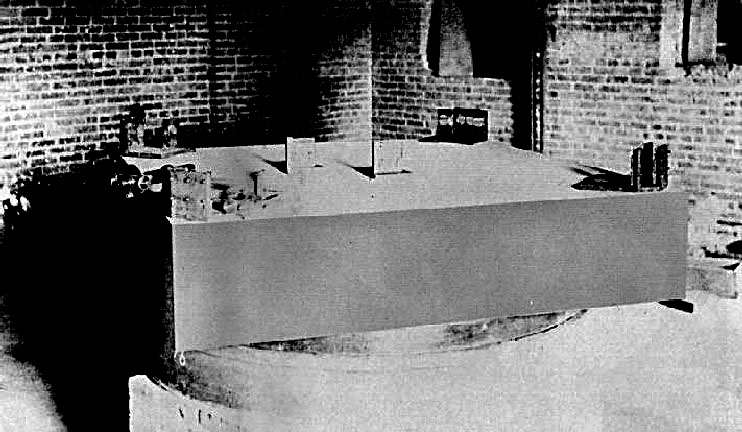
\includegraphics[width=\hsize]{chapters/images/MichelsonMorleyExperiment1887.jpg}
\caption{Das von Michelson und Morley gebaute Interferometer zur Messung
der Geschwindigkeit relativ zum Äther.
dDer Lichtstrahl wurde auf jedem Ast des Interferometers durch Spiegel
mehrmals hin und her reflektiert, um die scheinbare Länge der Arme
zu vergrössern.
Das Interferometer war auf einer grossen Steinplatte aufgebaut, die auf einem
Bad aus Quecksilber schwamm, um sie möglichst gut von Erschütterungen zu
isolieren.
\label{MMinterferometer}}
\end{figure}
Dies ist der Kontext, in dem Albert A.~Michelson und Edward W.~Morley
ihr berühmtes Interfero\-meter-Experiment durchführten.
Das Experiment vergleicht die Lichtausbreitung entlang zweier aufeinander
senkrecht stehender gleich langer Wege, indem es die Lichtwellen nach 
Durchlaufen der Wege zur Interferenz bringt
(Abbildung~\ref{skript:speziell:interferometerprinzip}).
Verändert sich die Laufzeit auch nur um einen Bruchteil einer Wellenlänge,
müsste dies dadurch erkennbar werden, dass sich die Interferenzmuster
verschieben.
Das von Michelson und Morley gebaute Instrument
(Abbildung~\ref{MMinterferometer}) wäre in der Lage
gewesen, eine Geschwindigkeitsänderung der Lichtgeschwindigkeit von
wenigen km/s festzustellen.
Beeinflusst der Äther die Lichtausbreitungsgeschwindigkeit, müsste 
man Betrag und Richtung der Äthergeschwindigkeit durch Drehen der
Aparatur um die vertikale Achse wie auch durch die Erddrehung
bestimmen können.

Im Michelson-Morley-Experiment wie auch in zahlreichen späteren, noch
genaueren Experimenten konnte keine Bewegung des Äthers festgestellt
werden.
Es gibt also keinen Hinweis darauf, dass es den Äther gibt und es
sieht so aus, als ob elektromagnetische Wellen für Ihre Ausbreitung
kein Medium brauchen.
Da auch sonst in der Elektrodynamik auch mit den präzisesten Messungen
keine Abweichungen von der Theorie festgestellt werden konnten,
ist die Galilei-Transformation
\eqref{skript:kruemmung:galileitransformation} wohl nur eine
Approximation ist.

Einstein hat diesen Schritt 1905 in seiner Arbeit \cite{skript:einstein}
vollzogen, seine Theorie wird heute die speziellen Relativitätstheorie genannt.
Ziel dieses Kapitels ist zu zeigen, welche Auswirkungen seine
Erkenntnis auf die Mechanik aber auch auf unser Weltbild hat.

\section{Lichtkegel}
\rhead{Lichtkegel}
Aus dem Michelson-Morley-Experiment weiss man, dass jeder Beobachter
die gleiche Lichtgeschwindigkeit $c$ im Vakuum misst.
Einstein hat die experimentell sehr gut bestätigte Konstanz der
Lichtgeschwindigkeit daher als Ausgangspunkt seiner Theorie genommen.
Entscheidend für die Physik ist, ob zwei Punkte sich mit elektromagnetischen
Wellen beeinflussen können.
Es ist daher nicht mehr ausreichend, nur Punkte miteinander zu vergleichen,
es muss auch immer die Zeit berücksichtigt werden, zu der sie verglichen
werden.
Raum und Zeit verschmelzen so zu einem einzigen vierdimensionalen
Kontinuum mit den Koordinaten $(t,x,y,z)$, welche wir die Raumzeit
nennen.
Quadrupel $(t,x,y,z)$ heissen auch {\em Ereignisse}.
\index{Ereignis}
Zwei Ereignisse $(t_1,x_1,y_1,z_1)$ und $(t_2,x_2,y_2,z_2)$ können
kausal voneinander abhängen, wenn ein Lichtsignal sich vom einen Ereignis
zum anderen Ereignis ausbreiten kann.
Dazu ist notwendig, dass der ``Abstand''
\begin{equation}
s^2
=
-c^2(t_1-t_2)^2
+
\mathstrut
\underbrace{
(x_1-x_2)^2
+
(y_1-y_2)^2
+
(z_1-z_2)^2}_{\displaystyle\text{Raumabstand}}
\label{skript:kruemmung:raumzeitabstand}
\end{equation}
gleich $0$ ist.
Breitet sich die Wirkung langsamer als mit Lichtgeschwindigket aus,
wird die zeitliche Differenz noch grösser sein, und damit der
Ausdruck~\eqref{skript:kruemmung:raumzeitabstand} negativ ist.

\begin{figure}
\centering
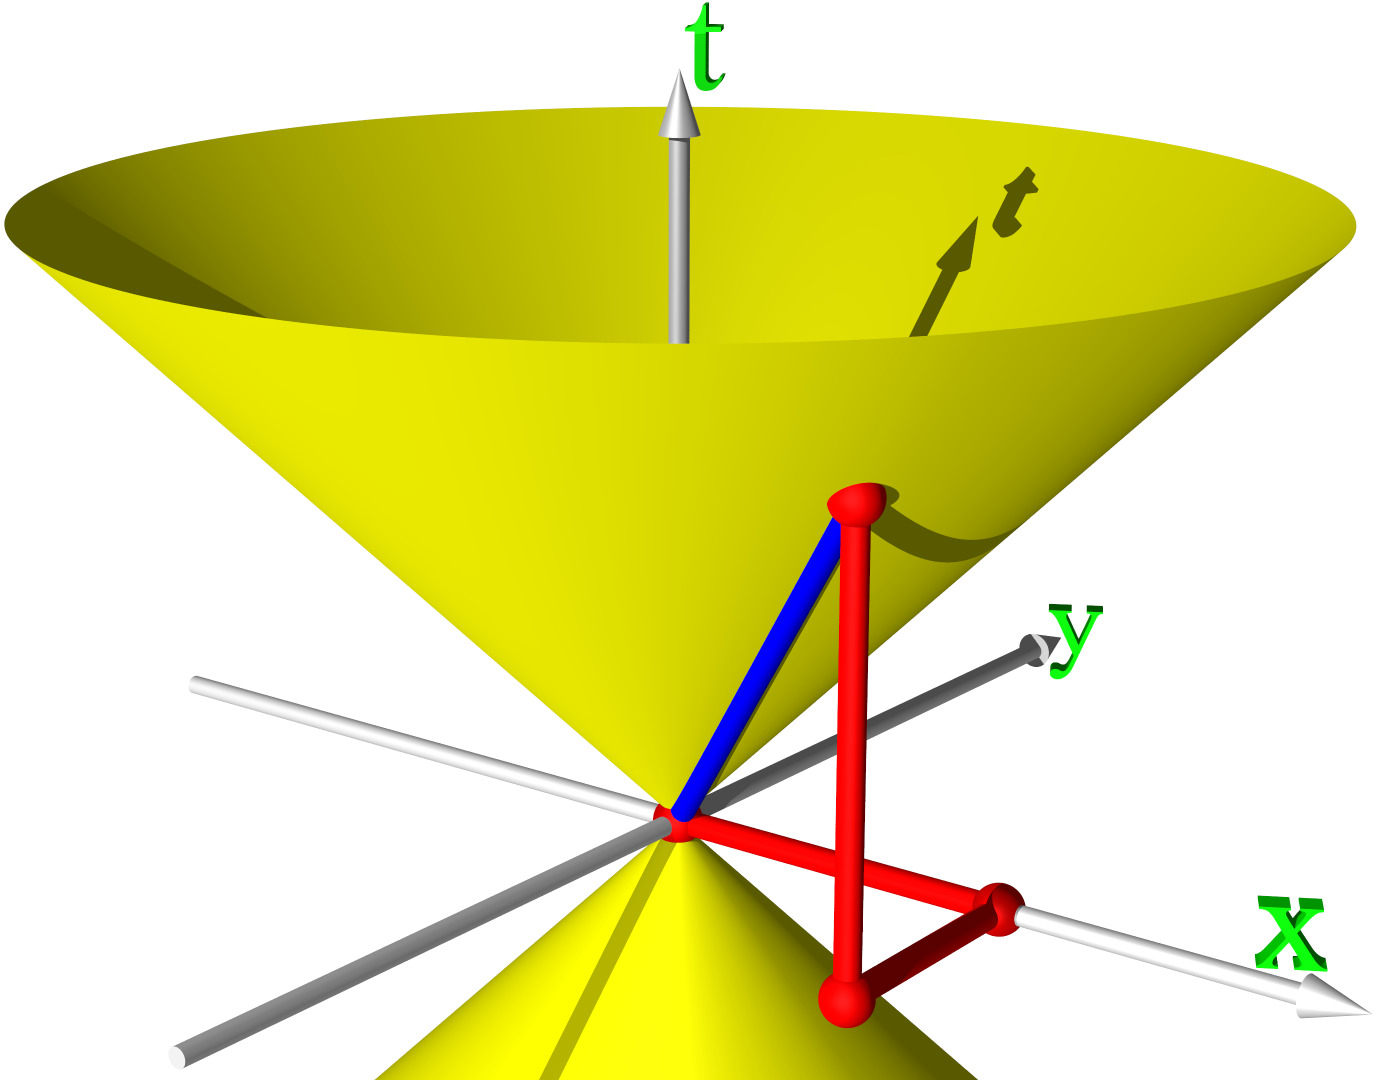
\includegraphics[width=\hsize]{chapters/3d/lichtkegel.jpg}
\caption{Lichtkegel ausgehend vom Nullpunkt zur Zeit $t=0$.
Alle Punkte innerhalb des Kegels mit $t>0$ liegen in der Zukunft des
Beobachters im Nullpunkt, solche mit $t<0$ in seiner Vergangenheit.
Punkte ausserhalb des Kegels können vom Nullpunkt aus nicht
beeinflusst werden.
Nur Punkte innerhalb des Kegels mit $t<0$ können Einfluss haben
auf den Nullpunkt.
\label{skript:kruemmung:fig:lichtkegel}}
\end{figure}

Das Vorzeichen des Ausdrucks~\eqref{skript:kruemmung:raumzeitabstand}
beschreibt also, ob zwei Ereignisse sich gegenseitig beeinflussen
können. 
Ist er negativ, dann ist eine Beeinflussung mit einer Wirkung möglich,
die sich weniger schnell als Licht ausbreitet.
Ist er gleich $0$, ist nur eine Beeinflussung mit einer Wirkung möglich,
die sich mit Lichtgeschwindigkeit ausbreitet.
Ist er positiv, ist keine gegenseitige Beeinflussung möglich.
Dies führt auf eine Unterteilung des Raumes in drei Gebiete
(Abbildung~\ref{skript:kruemmung:fig:lichtkegel}).
Die Fläche mit der Gleichung
\[
-c^2t^2+x^2+y^2+z^2=0
\]
heisst der Lichtkegel.
Ereignisse innerhalb des Lichtkegels mit $t>0$ können vom Nullpunkt aus
beeinflusst werden.
Ereignisse innerhalb des Lichtkegels imt $t<0$ können auf den Nullpunkt
Einfluss nehmen.
Alle anderen Ereignisse können den Nullpunkt weder beeinflussen
noch von ihm beeinflusst werden.
Sie müssen daher als die Gegenwart des Nullpunktes bezeichnet
werden.

Der Formalismus einer Metrik passt ganz hervorragend auf die hier
vorliegende Situation.
Verwenden wir als Koordinaten
\[
\begin{aligned}
x^0 &= ct,
&
x^1&=x,
&
x^2&=y,
&
x^3&=z,
\end{aligned}
\]
dann kann $s^2$ mit der Metrik
\begin{equation}
g_{\mu\nu}
=
\eta_{\mu\nu}
=
\begin{pmatrix}
-1&0&0&0\\
 0&1&0&0\\
 0&0&1&0\\
 0&0&0&1
\end{pmatrix},
\label{skript:speziell:metrik}
\end{equation}
der sogenannten
{\em Minkowski-Metrik}
\index{Minkowski-Metrik}
berechnet werden.
Die spezielle Relativitätstheorie beschreibt die Welt also einen
vierdimensionalen Raum, die Raum-Zeit, der Raumkoordinaten und Zeitkoordinate
in einem einzigen mathematischen Modell kombiniert.
Die Metrik~\eqref{skript:speziell:metrik} beschreibt dann die
Kausalitätsstruktur der Welt.

In diesem Bild gibt es also keinen sinnvollen Begriff der Gleichzeitigkeit
mehr.
Wäre das Universum nicht aus einem Punkt entstanden, wie das Big Bang-Modell
besagt, dann wäre bereits die Frage ``Wann ist das Universum entstanden''
unsinnig, denn es gibt keinen sinnvollen Art und Weise, wie etwas gleichzeitig
im ganzen Universum stattfinden könnte.
Diese Beobachtung hat zu Einsteins Zeit aber keine grossen Wellen
geworfen, denn die meisten Phyisker gingen davon aus, dass das Universum
ewig und statisch ist, dass es also gar keinen Anfang braucht.
Auch Einstein ging davon aus, was ihn später in seiner allgemeinene
Relativitätstheorie dazu gebracht hat, einen nicht weiter erklärbaren
Term hinzuzufügen, einzig um zu erreichen, dass das Universum statisch 
sein kann.

Wenn die Frage ``Wann ist das Universum entstanden'' überhaupt eine
sinnvolle Antwort haben soll, dann nur, wenn das Universum zur Zeit
der Entstehung nur ein Punkt gewesen ist.
Wenn das Universum ausgedehnt entstanden ist, dann ist die Frage
nach dem Entstehungszeitpunkt sinnlos.

\section{Zeitartige und raumartige Richtungen}
\rhead{Zeitartige und raumartige Richtungen}
Die Raumrichtungen $x^1$, $x^2$ und $x^3$ unterscheiden sich grundsätzlich
von der Zeitrichtung $x^0$.
Um diesem Unterschied Rechnung zu tragen, verwenden wir auch die Notation
$x^k$ mit einem lateinischen Index $k$ für die Koordinaten in Raumrichtung,
während $x^0$ die Zeitrichtung ist.

Allerdings ist diese Unterscheidung in Zeitkoordinate und Raumkoordinaten
für beliebige Koordinatensysteme nicht mehr sinnvoll.
Wir können aber immer noch Vektoren auf Grund des Vorzeichens der 
Metrik unterscheiden.
Ein Vierervektor $x^\mu$ auf dem Lichtkegel erfüllt $g_{\mu\nu}x^\mu x^\nu=0$.
Ein Vierervektor  mit $x^k=0$ und $x^0=ct$ erfüllt dagegen
\[
g_{\mu\nu} x^\mu x^\nu
=
g_{00}(x^0)^2 = -c^2 t^2<0.
\]
Man nennt einen Vektor $A^\mu$ zeitartig, wenn er $g_{\mu\nu}A^\mu A^\nu<0$ 
erfüllt.
Raumartig dagegen heisst ein Vektor $A^\mu$, für den
$g_{\mu\nu} A^\mu A^\nu>0$
gilt, wie zum Beispiel für einen Vektor mit $x^0=0$:
\[
g_{\mu\nu}x^\mu x^\nu
=
(x^1)^2
+
(x^2)^2
+
(x^3)^2
>0.
\]
Der Lichtkegel trennt also die zeitartigen Vektoren von den raumartigen
Vektoren.
Ein Ereignis kann ein anderes beeinflussen, wenn der Differenzvektor
zeitartig ist.
Insbesondere muss der Vektor zwischen zwei Punkten auf der Bahn 
eines Teilchens immer zeitartig sein.

\section{Lorentztransformation}
\rhead{Lorentztransformation}
Der Ausdruck~\eqref{skript:kruemmung:raumzeitabstand} ist nicht
invariant bei einer Galilei-Transformation.
Damit stellt sich die Frage, welche Transformationen denn
invariant wären.
Dies wären die Koordinaten-Änderungen, die zulässig sind, wenn
man das grundlegende Gesetz~\eqref{skript:kruemmung:raumzeitabstand}
der Kausalität erhalten will.

Zunächst sind Koordinatentransformationen, die nur die Raumkoordinaten
$x$, $y$ und $z$ beeinflussen, und den räumlichen Abstand nicht
ändern, zulässig.
Diese Transformationen sind aber wohlbekannt.
In der Linearen Algebra lernt man, dass genau die orthogonalen
Matrizen $A\in \textrm{O}(3)$, also Matrizen mit $A^tA=E$ diese
Eigenschaft haben.
Diese entsprechen räumlichen Drehungen und Spiegelungen.

Wenn sich aber zwei Koordinatensystem gegeneinander verschieben,
so wie bei der Galilei-Transformation, dann müssen auch die auch
die Zeitkoordinaten in die Transformation involviert sein.
Wir suchen also eine Koordinatentransformation, die nur die
$t$- und $x$-Koordinaten betrifft.
Wir können Sie in der Form
\begin{equation}
\begin{linsys}{3}
t'&=& a_{11}t&+&a_{12}x\\
x'&=& a_{21}t&+&a_{22}x
\end{linsys}
\end{equation}
ansetzen.
Wir verlangen jetzt aber, dass der
Ausdruck~\eqref{skript:kruemmung:raumzeitabstand}
unverändert bleibt.
Da die $y$- und $z$-Koordinaten ohnehin nicht involviert sind, bedeutet
das, dass
\begin{align*}
-c^2t^2 + x^2
&=
-c^2t'^2 + x'^2
\\
&=
-c^2(a_{11}t+a_{12}x)^2 + (a_{21}t+a_{22}x)^2
\\
&=
-c^2a_{11}^2t^2 -2c^2a_{11}a_{12}tx -c^2a_{12}^2x^2
+a_{21}^2t^2+2a_{21}a_{22}tx+a_{22}^2x^2
\\
&=
-(c^2a_{11}^2 - a_{21}^2)t^2
+2(-c^2a_{11}a_{12}+a_{21}a_{22})tx
+(-c^2a_{12}^2 + a_{22}^2)x^2.
\end{align*}
Da dies für beliebige Werte von $x$ und $t$ gelten muss, müssen die
Koeffizienten der beiden Seiten übereinstimmen. 
Wir erhalten damit für die Koeffizienten $a_{ik}$ die Gleichungen
\[
\begin{aligned}
c^2a_{11}^2-a_{21}^2&=c^2,
&&\Rightarrow&
a_{11}^2
-
\biggl(\frac{a_{21}}{c}\biggr)^2
&=1,
\\
-c^2a_{12}^2+a_{22}^2&=1,
&&\Rightarrow
&
a_{22}^2 - (ca_{12})^2&=1,
\\
a_{21}a_{22}&=c^2a_{11}a_{12}.
\end{aligned}
\]
Da die Differenz der Quadrate jeweils $1$ ist, können die Basen
als Werte des hyperbolischen Kosinus und Sinus dargestellt werden:
\[
\begin{aligned}
a_{11}&=\cosh\beta_1, &&&\frac{a_{21}}{c}&=\sinh\beta_1,
\\
a_{22}&=\cosh\beta_2,&&&ca_{12}&=\sinh\beta_2.
\end{aligned}
\]
Die dritte Gleichung lautet dann
\begin{align*}
a_{21}a_{22}=c\sinh\beta_1\cosh\beta_2
&=
c^2a_{11}a_{12}=c^2\cosh\beta_1\frac1c\sinh\beta_2
\\
c\sinh\beta_1\cosh\beta_2
&=
c\cosh\beta_1\sinh\beta_2
\\
\tanh\beta_1&=\tanh\beta_2,
\end{align*}
es folgt $\beta_1=\beta_2$, wir schreiben dafür im Folgenden einfach
nur $\beta$.
Damit haben wir die gesuchte Transformation gefunden, es ist
\begin{equation}
\begin{pmatrix}
a_{11}&a_{12}\\
a_{21}&a_{22}
\end{pmatrix}
=
\begin{pmatrix}
 \cosh\beta&\frac1c\sinh\beta\\
c\sinh\beta&\cosh\beta
\end{pmatrix}
\end{equation}
Um die physikalische Bedeutung des Parameters $\beta$ zu verstehen, 
betrachten wir die Punkte $x=0$ für beliebige $t$.
Sie werden abgebildet auf
\[
\begin{aligned}
x' &= c\sinh\beta \cdot t,
&
&&
t' &=  \cosh\beta \cdot t.
\end{aligned}
\]
Der Quotient dieser beiden Ausdrücke ist die Geschwindigkeit
\[
v = c\frac{\sinh\beta}{\cosh\beta}
\qquad\Rightarrow\qquad
\frac{v}{c}
=
\tanh\beta,
\]
mit der sich der Nullpunkt des $t$-$x$-Systems im $t'$-$x'$-System
bewegt.

Nach den Formeln im Abschnitt~\ref{skript:sinh:section:abh} kann 
man jetzt auch $\sinh\beta$ und $\cosh\beta$ durch $v/c$ ausdrücken.
Setzen wir ein, erhalten wir
\[
\begin{aligned}
\sinh\beta
&=
\frac{\tanh\beta}{\sqrt{1-\tanh^2\beta}}
=
\gamma\cdot\frac{v}{c}
&
&\text{mit}&
\gamma = \frac{1}{\displaystyle\sqrt{1-\biggl(\frac{v}{c}\biggr)^2}}
\qquad\text{und}
\\
\cosh\beta
&=
\frac1{\sqrt{1-\tanh^2\beta}}
=
\gamma.
\end{aligned}
\]

Der Parameter $\tanh\beta$ hat also die Bedeutung einer in Einheiten
der Lichtgeschwindigkeit gemessenen Geschwindigkeit.
Da also $v/c=\tanh\beta$ ist, kann man die Transformation auch
als
\begin{equation}
\begin{pmatrix}
a_{11}&a_{12}\\
a_{21}&a_{22}
\end{pmatrix}
=
\frac{1}{\gamma}
\begin{pmatrix}
\displaystyle 1
	& \displaystyle\frac{v}{c^2}
\\
\displaystyle v
	&\displaystyle 1
\end{pmatrix}
\label{skript:kruemmung:lorentz}
\end{equation}
schreiben.
Die Transformation 
\eqref{skript:kruemmung:lorentz}
heisst {\em Lorentz-Transformation}.
\index{Lorentz-Transformation}

Befindet sich ein Beobachter im ursprünglichen $t$-$x$-System in Ruhe
im Nullpunkt, dann ist seine Zeitkoordinate im $t'$-$x'$-System
\begin{equation}
t'=t\cdot\gamma = \frac{t}{\displaystyle\sqrt{1-\biggl(\frac{v}{c}\biggr)^2}},
\label{skript:speziell:zeitdilatation}
\end{equation}
der Lauf der Zeit ist in den beiden Koordinatensystemen verschieden.
Im $t'$-$x'$-Koordinatensystem läuft die Zeit um den Faktor $\gamma$
gedehnt.
Umgekehrt gilt natürlich auch $t=t'/\gamma$.


Die Darstellung \eqref{skript:kruemmung:lorentz} der Lorenztransformation
ist nicht sehr symmetrisch.
Dies liegt daran, dass die Zeit-Koordinate eine ganz andere Masseinheit
verwendet.
Schreibt man für die Koordinaten 
\[
\begin{aligned}
x^0&=ct,&
x^1&=x,&
x^2&=y,&
x^3&=z&
\end{aligned}
\]
dann wird die Lorentztransformation
\begin{equation}
\begin{pmatrix}
x^{\prime0}\\
x^{\prime1}\\
x^{\prime2}\\
x^{\prime3}
\end{pmatrix}
=
\begin{pmatrix}
\displaystyle          \gamma &\displaystyle\frac{v}{c}\gamma& 0 & 0 \\
\displaystyle\frac{v}{c}\gamma&\displaystyle           \gamma& 0 & 0 \\
      0                       &                              & 1 & 0 \\
      0                       &                              & 0 & 1 
\end{pmatrix}
\begin{pmatrix}
x^0\\x^1\\x^2\\x^3
\end{pmatrix}.
\label{skript:speziell:4lorentz}
\end{equation}
In dieser Form ist die Lorentztransformation klar symmetrischer.

\section{Weltlinien und Eigenzeit}
\rhead{Weltlinien und Eigenzeit}
Die Bewegung eines Teilchens in der Raum-Zeit ist eine Kurve
$(t(s), x(s), y(s), z(s))$
mit dem Parameter $s$, die man auch {\em Weltlinie} nennt.
\index{Weltlinie}
Da sich das Teilchen nicht mit Lichtgeschwindigkeit bewegen kann, muss
für den Tangentialvektor 
\[
-c^2\dot t(s)^2
+ \dot x(s)^2 + \dot y(s)^2 + \dot z(s)^2
<
0
\]
gelten, darin bezeichnet der Punkt die Ableitung nach dem 
Parameter $s$.
Offenbar bewegt sich das Teilchen mit der Geschwindigkeit
\[
v^2 = \frac{\dot x(s)^2 + \dot y(s)^2 + \dot z(s)^2}{\dot t(s)^2}
\]
durch die Raumzeit.
Da sich das Teilchen bewegt, läuft die Zeit in einem Koordinatensystem,
das sich mit dem Teilchen mitbewegt, um den Faktor
\eqref{skript:speziell:zeitdilatation}
langsam.
Setzt man die Definitionen ein, erhält man
\begin{align*}
\frac{1}{\gamma}
=
\sqrt{1-\frac{v^2}{c^2}}
&=
\sqrt{1- \frac{\dot x(s)^2 + \dot y(s)^2 + \dot z(s)^2}{c^2\dot t(s)^2}}
\\
&=
\sqrt{-(-c^2\dot t(s)^2+\dot x(s)^2 + \dot y(s)^2 + \dot z(s)^2)}\frac{1}{c\dot t(s)}.
\end{align*}
Die im bewegten Koordinatensystem gemessene Zeit ist
\begin{align*}
\int\frac{1}{\gamma}\,dt
&=
\int
\sqrt{1-\frac{v^2}{c^2}}\,dt
=
\int
\sqrt{-(-c^2\dot t(s)^2+\dot x(s)^2 + \dot y(s)^2 + \dot z(s)^2)}\frac{1}{c\dot t(s)}
\,dt
\\
&=
\int
\sqrt{-(-c^2\dot t(s)^2+\dot x(s)^2 + \dot y(s)^2 + \dot z(s)^2}\frac{1}{c\dot t(s))}
\dot t(s)\,ds
\\
&=
\int
\frac1c
\sqrt{-(-c^2\dot t(s)^2+\dot x(s)^2 + \dot y(s)^2 + \dot z(s)^2)}
\,ds.
\end{align*}
In $x^\mu$-Koordinaten bedeutet dies, dass
\begin{equation}
\tau
=
\int
\frac{1}{\gamma}\,dt
=
\int
\sqrt{1-\frac{v^2}{c^2}}\,dt
=
\frac1{c}
\int
\sqrt{-g_{\mu\nu}\dot x^\mu(s) \dot x^\nu(s)}\,ds
\label{skript:speziell:eigenzeit}
\end{equation}
die Zeit ist, die entlang der Kurve $x^\mu(s)$ für den
mitbewegten Beobachter vergangen ist.
Man nennt $\tau$ die {\em Eigenzeit} des
Beobachters, der sich entlang der Weltlinie $x^\mu(s)$ bewegt.
\index{Eigenzeit}
Da der Integrand in~\eqref{skript:speziell:eigenzeit} unabhängig ist
vom Koordinatensystem, ist $\tau$ ebenfalls unabhängig vom Koordinatensystem.

\section{Energie und Impuls}
\rhead{Energie und Impuls}
Ein Teilchen der Masse $m$, die im Nullpunkt ruht, hat keinen
Impuls.
In einem anderen Koordinatensystem nimmt hat das Teilchen dagegen
eine Geschwindigkeit, und damit auch einen Impuls.
Dies zeigt, dass eine koordinatensystemunabhägngige Beschreibung
nicht nur mit dem Impuls funktionieren kann.
Wir brauchen eine erweiterte Erhaltungsgrösse, die wir zur Beschreibung
der Bewegung eines Teilchens verwenden können.

Die Kurve $x^\mu(s)$ und die Ableitung nach dem Kurvenparameter sind
offenbar keine geeigneten Grössen, denn der Kurvenparameter ist
keine vom Koordinatensystem unabhängige Grösse.
Die Eigenzeit ist aber eine solche koordinatensystemunabhängige
Grösse, wir schliessen daraus, dass die Ableitung der Position
nach der Eigenzeit, die sogenannte Vierergeschwindigket, der einzig
sinnvolle Ersatz für die Geschwindigkeit.
Da die Eigenzeit auch im Wesentlichen die Bogenlänge ist, führt die
Ableitung automatisch auf einen Einheitsvektor.

Ein ruhendes Teilchen hat die Weltlinie
\[
t\mapsto (t, x, y, z)=(t,0,0,0),
\]
der Parameter ist die Koordinatenzeit.
Da das Teilchen keine Geschwindigkeit hat, ist $t$ auch die Eigenzeit,
und die Vierergeschwindgkeit $u^\mu$ ist der Vektor mit den
Komponenten
\[
\begin{aligned}
u^0 &= c,
&&&
u^1&=u^2=u^3 = 0.
\end{aligned}
\]
Seine Länge gemessen mit der Metrik ist
\[
g_{\mu\nu}u^\mu u^\nu=-c^2,
\]
sie ist eine koordinatensystemunabhängige Grösse.

Wendet man darauf eine Lorentztransformation mit Geschwindigkeit $v$ an,
erhält man den Vektor
\[
\begin{aligned}
u^0
&=
c\gamma,
&
u^1
&=
\frac{v}{c}\gamma c
=v\gamma
&&\text{und}
&
u^2&=u^3=0.
\end{aligned}
\]
Wir rechnen das Skalarprodukt mit Hilfe der Metrik nach:
\[
-(u^0)^2 + (u^1)^2 + (u^2)^2 + (u^3)^2
=
-c^2\gamma^2 + v^2\gamma^2
=
-c^2\gamma^2
\underbrace{\biggl(1-\frac{v^2}{c^2}\biggr)}_{\displaystyle=\frac{1}{\gamma^2}}
=
-c^2.
\]

Multiplizieren wir die Vierergeschwindigkeit mit $m$, erhalten wir
den sogenannten Viererimpuls $p^\mu = mu^\mu$.
Der Betrag des Viererimpulses ist eine Konstante, es gilt
\[
g_{\mu\nu}p^\mu p^\nu
=
-
m^2\gamma^2 c^2
+
m^2 \gamma^2 v^2
=
-m^2c^2\biggl(\displaystyle 1-\frac{v^2}{c^2}\biggr)\gamma^2
=
-m^2c^2.
\]
Die Raumkomponenten $p^1$, $p^2$ und $p^3$ haben eine offensichtliche
Interpretation in der Newtonschen Mechanik.
Bis auf den Faktor $\gamma$ stimmten die Raumkomponenten des Viererimpulses
mit dem Newtonschen Impuls überein.
Schreiben wir $M=m\gamma$, dann wird sogar $p^k = M v^k$, d.~h.~die
Raumkomponenten des Viererimpulses stimmen mit dem Newtonschen Impuls 
für die Masse $M=m\gamma  \ge m$ "uberein.
$M=m\gamma$ heisst die relativistische Masse.
Eine bewegte Masse ist also grösser als eine ruhende.

Um die Bedeutung der $0$-Komponente des Viererimpulses besser zu
verstehen, entwickeln wir ihn für kleine Geschwindigkeiten.
Dazu verwenden wir die Potenzreihe
\[
\frac1{\sqrt{1-x}}
=
1+\frac12x+\frac{1\cdot 3}{2\cdot 4}x^2 + \frac{1\cdot 3\cdot 5}{2\cdot 4\cdot 6}x^3+\dots,
\]
die man aus der binomischen Reihe\footnote{%
Die {\em binomische Reihe} für negative Exponenten ist die Reihe
\[
(1\pm x)^{-m}
=
1\mp mx +\frac{m(m+1)}{2!}x^2 \mp \frac{m(m+1)(m+2)}{3!} x^3 +\dots
\]
mit $m>0$.
\index{binomische Reihe}
} für negative Exponenten ableiten kann.
Setzen wir hier für $x$ den Quotienten $(v/c)^2$ ein, erhalten wir
\[
Mc
=
m\gamma c
=
\frac{m}{\sqrt{1-\displaystyle\frac{v^2}{c^2}}} c
=
mc\biggl(1+\frac12\cdot\frac{v^2}{c^2}+\dots\biggl)
\]
Multipliziert man mit $c$, erhält man 
\[
u^0c = mc^2 + \frac12mv^2+\dots
\]
Der zweite Term ist die wohlbekannte kinetische Energie.
Der erste Term bleibt gleich gross, auch wenn die Masse sich
nicht bewegt.
Wir müssen diesen Term daher als eine Energie interpretieren, die
zu der Masse gehört unabhängig von deren Bewegungszustand.
Wir dürfen diese Energie nicht einfach subtrahieren, denn dadurch
würde das Transformationsgesetz für den Viererimpuls bei einer
Lorentztransformation verletzt.
Die Energie
\begin{equation}
E=mc^2
\label{E=mc2}
\end{equation}
heisst die {\em Ruheenergie} der Masse $m$.
\index{Ruheenergie}

\section{Energie-Impuls-Tensor}
\rhead{Energie-Impuls-Tensor}
Die Betrachtungen zum Viererimpuls und zur Energie haben gezeigt, dass
Masse und Geschwindigkeit nicht unabhängig voneinander betrachtet
werden können.
Andererseits zeigt das newtonsche Gravitationsgesetz, dass sich Schwerkraft
von der Masse eines Körpers ausgeht.
Die Newtonsche Theorie ist daher schon im Ansatz nicht der
speziellen Relativitätstheorie verträglich.
Die Masse allein kann bestensfalls in einem Koordinatensystem als
Quelle der Schwerkraft dienen, in dem die Masse ruht.
Eine modifizierte Theorie muss daher als Quelle für die Gravitation
ein Objekt verwenden, welches wie der Vierimpuls unahängig vom
Bewegungszustand definiert werden kann.

Auch genügt es nicht, nur Massepunkte zu studieren, da die meisten
Objekt des Universums ausgedehnt sind.
In der Newtonschen Theorie wird daher das von einer Masseverteilung mit
Dichte $\varrho(x,y.z)$ verursachte Gravitationsfeld studiert.
In der verallgemeinerten Theorie reicht die Dichte nicht aus,
wir müssen zulassen, dass die Materie sich bewegt, was wir mit einem
Stromdichtevektor $\vec j$ abbilden können.
Die relativistische Grösse dazu wäre der Vierervektor der Impulsdichte
bestehend aus den Komponenten $j^\mu=\varrho u^\mu$,
wobei $u^\mu$ die Komponenten der Vierergeschwindigkeit des Gases sind.

Gesucht ist jetzt also eine Grösse, die zu jeder Zeit und in jedem
Punkt des Raumes den Viererimpuls der dort vorhandenen Materie zu
berechnen.
Im Ruhesystem des Gases reicht die Dichte des Gases zur Beschreibung.
In einem bewegten System wird man aber feststellen, dass das Gas auch
noch Impuls trägt, der ebenfalls berücksichtigt werden muss.
Die gesuchte Grösse muss also erlauben, den Viererimpuls-Inhalt eines
räumlich und zeitlich begrenzten Gebietes zu bestimmen, einer ``Box'', 
die dadurch beschrieben werden kann, dass alle Koordinaten ein einem
Intervall
\[
a^\mu \le x^\mu \le b^\mu
\]
bleiben.
Wechselt man in ein bewegtes Koordinatensystem, wird sich diese
gleiche Box gegenüber dem Koordinatensystem bewegen.
Die gesuchte Grösse muss also in der Lage sein, den Viererimpuls-Inhalt
der Box auch dann zu berechnen, wenn sich die Box bewegt.

Statt den Inhalt der Box zu berechnen, können wir auch die Änderung des
Inhalts der Box berechnen, die dadurch entsteht, dass Viererimpuls durch
die Wände der Box strömt.
Eine Wand können wir dadurch beschreiben, dass dort eine der Koordinaten
konstant ist, also durch einen Standardbasisvektor, oder durch einen
Koordinatenindex.
Zu jeder Koordinate $\mu$ gibt es also den Vektor des Viererimpulses
\[
T^{\mu\nu}
\]
der durch die zu $\mu$ gehörende Seitenfläche fliesst.

Um dieses Konzept zu illustrieren beschränken wir uns für den Moment
auf zwei Dimensionen, also auf die Koordinaten $x^0=ct$ und $x^1=x$.
Eine Box ist ein Rechteck, die Kanten des Rechtecks sind definiert
dadurch, dass $x^0$ bzw.~$x^1$ konstant sind.
Betrachten wir zuerst den Fall $\mu=0$.
Dann ist $T^{\nu0}$ der Viererimpuls, der durch ein räumliches
Einheitsinterval fliesst.
Insbesondere ist $T^{00}$ der Fluss der Energiedichte durch das Interval,
$T^{10}$ ist der Impulsfluss durch das Interval.
Für $\mu=1$ ist $T^{01}$ die Energie, die in einem Einheitszeitinterval
durch die Koordinaten $x^1$ fliesst, und $T^{11}$ ist der Impuls, der in der
gleichen Zeit durch den Punkt $x^1$ fliesst.
Man beachte, dass die Masseinheiten
\[
\text{Energiefluss}
=
\frac{\text{Energie}}{\text{Länge}}
=
\frac{\text{kg}\frac{\text{m}^2}{\text{s}^2}}{\text{m}}
=
\frac{\text{kg}\cdot\text{m}}{\text{s}^2}
=
\frac{\text{kg}\frac{\text{m}}{\text{s}}}{\text{s}}
=
\frac{\text{Impuls}}{\text{Zeit}}
=
\text{Impulsstrom}
\]
erfüllen.
Ausserdem ist 
\[
\frac{\text{Impuls}}{\text{Zeit}}
=
\frac{\text{kg}\frac{\text{m}}{\text{s}}}{\text{s}}
=
\frac{\text{kg}\cdot\text{m}}{\text{s}^2},
\]
dies ist die Masseinheit des Druckes oder einer Spannung.
Wir können daher die Matrix $T^{\nu\mu}$
durch
\[
T^{\mu\nu}
=
\begin{pmatrix}
\text{Energiedichte}
&\text{Energiefluss}
\\
\text{Impulsdichte}
&\text{Impulsfluss = Druck}
\end{pmatrix}
\]
charakterisieren.
$T^{\mu\nu}$ heisst der {\em Energie-Impuls-Tensor}.
Er codiert die Information über den im Universum vorhandenen
Viererimpuls.

\index{Energie-Impuls-Tensor}

\subsection{Energie-Impuls-Tensor eines idealen Gases}
Ein ideales Gas ist isotrop, Kräfte wirken alle in die gleiche
Richtung.
Der Energie-Impuls-Tensor des ruhenden Gases muss daher durch die
Dichte $\varrho$ des Gases und den Druck $p$ beschrieben werden können.
Da sich das Gas nicht bewegt, fliesst kein Impuls durch eine Fläche
in Zeitrichtung.
Daher gilt
\[
T^{00}
=
\varrho
\qquad
\text{und}
\qquad
T^{k0}
=
0.
\]
Da sich das Gas nicht bewegt, fliesst auch keine Energie durch räumliche
Wände einer Box, so dass auch $T^{0k}=0$ gilt.
Da in einem idealen Gas keine Spannungen herschen, muss $T^{ik}$ diagonal
sein, und $T^{ik}=p$.
Also ist
\[
T^{ik}
=
\begin{pmatrix}
\varrho&0&0&0\\
0&p&0&0\\
0&0&p&0\\
0&0&0&p
\end{pmatrix}
\]
der Energie-Impuls-Tensor eines ruhenden idealen Gases mit Dichte
$\varrho$ und Drucke $p$.

Um daraus den Energie-Impuls-Tensor eines idealen in einem
beliebigen, möglicherweise auch bewegten Koordinatensystem zu
finden, müssen wir diesen Tensor aus dem Viererimpuls $u^\mu$
des Gases und möglicherweise aus dem metrischen $g^{\mu\nu}$ Tensor
zusammenbauen.
Wir behaupten, der gesuchte Tensor sei
\begin{equation}
T^{\mu\nu}
=
p g^{\mu\nu} + (p + \varrho)u^\mu u^\nu.
\label{skript:speziell:idealesgas}
\end{equation}
In der Tat ist für ein ideales Gas in Ruhe $u^0=1$ und $u^k=0$ und damit
$u^\mu u^\nu=0$ ausser wenn $\mu=\nu=0$.
Setzt man dies ein, erhält man
\begin{align*}
T^{00}
&=
pg^{00} + (p+\varrho) = -p+p+\varrho=\varrho
\\
T^{k0}
&=0
\\
T^{kl}
&=
p\delta^{kl}
+
(p+\varrho)\cdot 0
=
p\delta^{kl}.
\end{align*}
Der Ausdruck~\eqref{skript:speziell:idealesgas} ist ein Tensor, der
im Ruhesystem des Gases mit dem korrekten Energie-Impuls-Tensor
übereinstimmt,
daher ist er die allgemeine Form für den Energie-Impuls-Tensor.

\subsection{Energie-Impuls-Erhaltung}
In einem kräftefreien System sind Energie und Impuls erhalten, wir
möchten diese Aussage auch in unserem vierdimensionalen Formalismus
ausdrücken können.

\subsubsection{Kontinuitätsgleichung}
Betrachten wir zunächst die Strömung eines Mediums in drei Dimensionen.
Materie kann nicht einfach entstehen oder zerstört werden, dafür muss
es einen mathematischen Ausdruck geben.
Sei $\varrho(x,y,z,t)$ die Dichte des Mediums und $\vec v(x,y,z,t)$ 
seine Geschwindigkeit.
Wir berechnen, wie sich die Masse des Mediums in einem kleinen
Quader mit Seitenlängen $(\Delta x, \Delta y, \Delta z)$ in einem
Zeitinterval $\Delta t$ verändert.
In diesem Zeitinterval fliesst durch die Seitenwände senkrecht zur
$x$-Achse bei $x$ und $x+\Delta x$ 
Materie mit der Masse
\begin{align*}
m_x
&=
\varrho(x+\Delta x,y,z,t) v_x(x+\Delta x,y,z,t) F_x\,\Delta t
-\varrho(x,y,z,t) v_x(x,y,z,t) F_x\,\Delta t
\\
&=
\bigl(\varrho(x+\Delta x,y,z,t)
v_x(x+\Delta x,y,z,t) -\varrho(x,y,z,t) v_x(x,y,z,t)\bigr) F_x\,\Delta t
\\
&\simeq
\frac{\partial \varrho v_x}{\partial x}(x,y,z,t)\Delta x\, F_x\,\Delta t,
\end{align*}
wobei $F_x=\Delta x\,\Delta y$ der Flächeninhalt der Seitenfläche senkrecht
auf $x$ ist.

Dasselbe passiert durch die anderen Wände, so dass
die gesamte Masseänderung im Zeitinterval $\Delta t$
\[
\Delta m
=
\biggl(
\frac{\partial\varrho v_x}{\partial x}
+
\frac{\partial\varrho v_y}{\partial y}
+
\frac{\partial\varrho v_z}{\partial z}
\biggr)V\Delta t
\]
ist, darin ist $V$ das Volumen des Quaders.
Aus der Dichte können wir die Masseänderung aber auch berechnen,
es ist
\[
\Delta m
=
\frac{\partial\varrho}{\partial t}V \Delta t.
\]
Zusammen erhalten wir die Gleichung
\[
\frac{\partial\varrho}{\partial t}V \Delta t
=
\biggl(
\frac{\partial \varrho v_x}{\partial x}
+
\frac{\partial \varrho v_y}{\partial y}
+
\frac{\partial \varrho v_z}{\partial z}
\biggr)V\Delta t
\]
oder nach Division durch $V\Delta t$:
\begin{equation}
\frac{\partial\varrho}{\partial t}
-
\frac{\partial \varrho v_x}{\partial x}
+
\frac{\partial \varrho v_y}{\partial y}
+
\frac{\partial \varrho v_z}{\partial z}
=0.
\label{skript:speziell:kontinuitaetsgleichung}
\end{equation}
Die Gleichung~\eqref{skript:speziell:kontinuitaetsgleichung} heisst
{\em Kontinuitätsgleichung}.
\index{Kontinuitätsgleichung}
Schreiben wir $\vec j = \varrho\vec v$ und
\begin{equation}
\operatorname{div}\vec a
=
\frac{\partial a_x}{\partial x}
+
\frac{\partial a_y}{\partial y}
+
\frac{\partial a_z}{\partial z},
\label{skript:speziell:divergenz}
\end{equation}
für ein beliebiges Vektorfeld $\vec a$,
dann kann die Kontinuitätsgleichung auch sehr kompakt als
\[
\frac{\partial\varrho}{\partial t}-\operatorname{div}\vec j=0
\]
geschrieben werden.
Die Grösse $\operatorname{div}\vec a$ heisst die {\em Divergenz}
des Vektorfeldes $\vec a$.
\index{Divergenz}
Die Kontinuitätsgleichung~\eqref{skript:speziell:divergenz} drückt
die Erhaltung der Masse aus.

\subsubsection{Kontinuitätsgleichung für den Viererimpuls}
Verwenden wir jetzt wieder Koordinaten $x^\mu$, dann nimmt die
Kontinuitätsgleichung~\eqref{skript:speziell:divergenz}
die Form
\begin{align*}
0
&=
-
\frac{\partial \varrho}{\partial t}
+
\frac{\partial \varrho v_x}{\partial x}
+
\frac{\partial \varrho v_y}{\partial y}
+
\frac{\partial \varrho v_z}{\partial y}
\\
&=
-\frac{\partial c \varrho}{\partial x^0}
+\frac{\partial u^1}{\partial x^1}
+\frac{\partial u^2}{\partial x^2}
+\frac{\partial u^3}{\partial x^3}
=
\frac{\partial u^\mu}{\partial x^\mu}
\end{align*}
für die Viererimpulsdichte $u^\mu$ an.
Der Erhaltungssatz für den Viererimpuls kann daher
geschrieben werden als
\[
\frac{\partial T^{\mu\nu}}{\partial x^\mu}
=0
\]
in beliebigen Koordinaten.
Ist $A^{\mu}$ ein Vierervektor, dann ist
\[
\frac{\partial A^\mu}{\partial x^\mu}=0
\]
der allgemeine Ausdruck dafür, dass die Grösse $A^0$ und der zugehörige
Strom $A^k$ erhalten bleiben.

\subsection{Symmetrie des Energie-Impuls-Tensors}
Der Energie-Impuls-Tensor ist symmetrisch, dies kann man wie folgt einsehen.
Wir betrachten einen kleinen Würfel mit Kantenlänge $L$.
Die Komponenten $T^{ik}$ des Energie-Impuls-Tensors beschreiben die
$i$-Komponenten der Kräfte auf den $k$-Flächen des Würfels.
Insbesondere ist das Drehmoment um die $3$-Achse
\begin{align*}
M^{12}
&=
-T^{12}L^2(L/2) + T^{12}L^2 (-L/2)
\\
&\phantom{\mathstrut=}-(-T^{21}L^2)(L/2)-(T^{21}L^2)(-L/2)
\\
&=(T^{12}-T^{21})L^3
\end{align*}
Das Trägheitsmoment des Würfels ist proportional zu $L^5$,
die Winkelbeschleunigung des Würfels ist daher proportional
zu $(T^{12}-T^{21})L^{-2}$, was für $L\to 0$ beliebig gross würde.
ein beliebig kleiner Würfel würde daher zu beliebig grossen 
Drehgeschwindigkeit beschleunigt.
Da dies nicht sein kann, folgt $T^{12}-T^{21}=0$ oder allgemeine
\[
T^{\mu\nu}=T^{\nu\mu}.
\]



